\subsection{Continuous Simulation Extension (CSE): Tilt-Bound}
\frame{\tableofcontents[currentsubsection]}

\begin{frame}{Main Task: Find Type I Error at $\theta$}
\begin{figure}
    \centering
    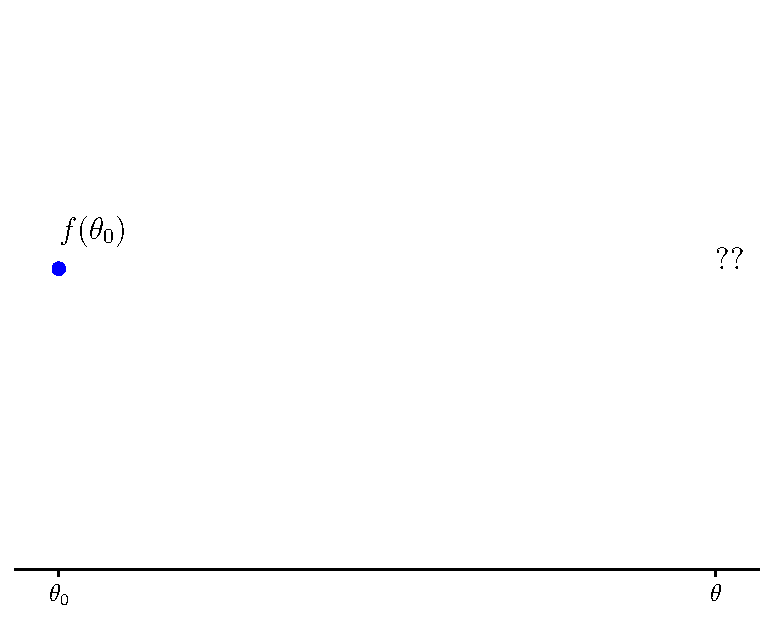
\includegraphics[width=0.75\linewidth]{figs/cse_problem.pdf}
\end{figure}
\begin{itemize}
    \item $X \sim P_\theta$ (known distribution), null space $\Theta$.
    \item Any arbitrary design $\design$.
    \item $f(\theta) := \prob_\theta\pr{\design \text{ rejects}}$.
\end{itemize} 
\end{frame}

\begin{frame}{Main Task: Find \textbf{Upper Bound} of Type I Error at $\theta$}
\begin{figure}
    \centering
    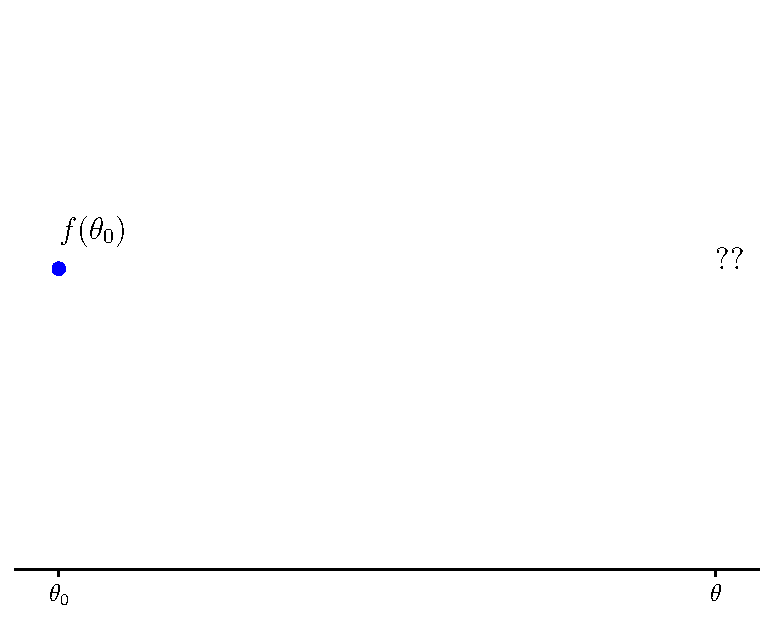
\includegraphics[width=0.75\linewidth]{figs/cse_problem.pdf}
\end{figure}
\begin{itemize}
    \item $X \sim P_\theta$ (known distribution), null space $\Theta$.
    \item Any arbitrary design $\design$.
    \item $f(\theta) := \prob_\theta\pr{\design \text{ rejects}}$.
\end{itemize} 
\end{frame}

\begin{frame}{Main Task: Find \textbf{Upper Bound} of Type I Error at $\theta$}
\begin{figure}
    \centering
    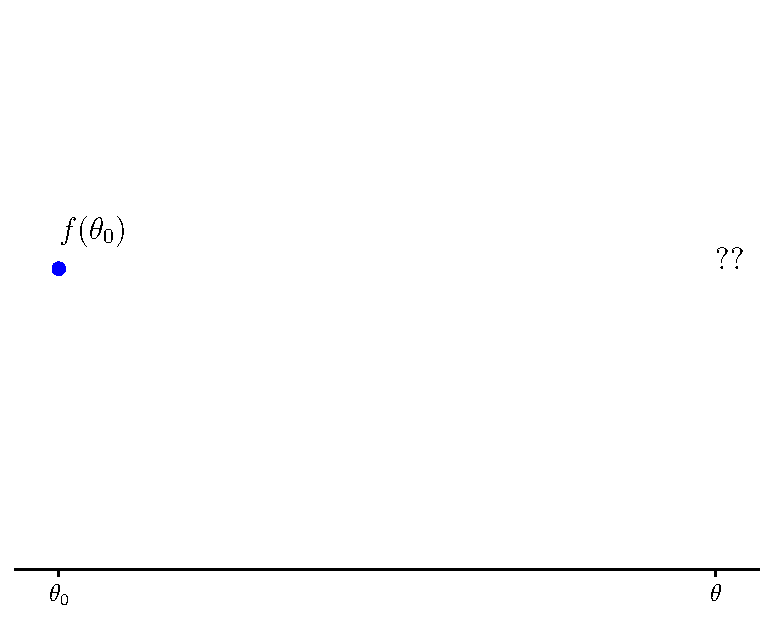
\includegraphics[width=0.75\linewidth]{figs/cse_problem.pdf}
\end{figure}
\begin{itemize}
    \item Assume further that $P_\theta$ is an \textbf{exponential family}.
    \item Does this help?
\end{itemize}
\end{frame}

\begin{frame}{Main Task: Find \textbf{Upper Bound} of Type I Error at $\theta$}
\begin{figure}
    \centering
    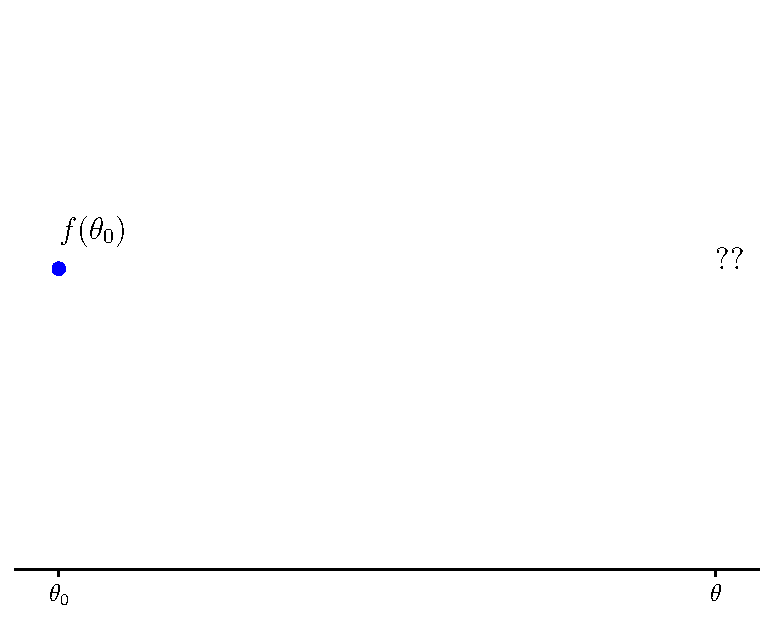
\includegraphics[width=0.75\linewidth]{figs/cse_problem.pdf}
\end{figure}
\begin{itemize}
    \item Assume further that $P_\theta$ is \textbf{Gaussian}.
    \item Does this help?
\end{itemize}
\end{frame}

\begin{frame}{Intuition for Upper Bounding the Type I Error}
\begin{itemize}
    \item \textbf{Morally}, distribution assumptions \emph{should} help!
    \item Use \textbf{``curvature''} information in distribution.
    \item \textbf{Restrict} the possible values for $f(\theta)$.
\end{itemize} 
\end{frame}

\begin{frame}{Claim: Upper Bound on the Type I Error}
\begin{figure}
    \centering
    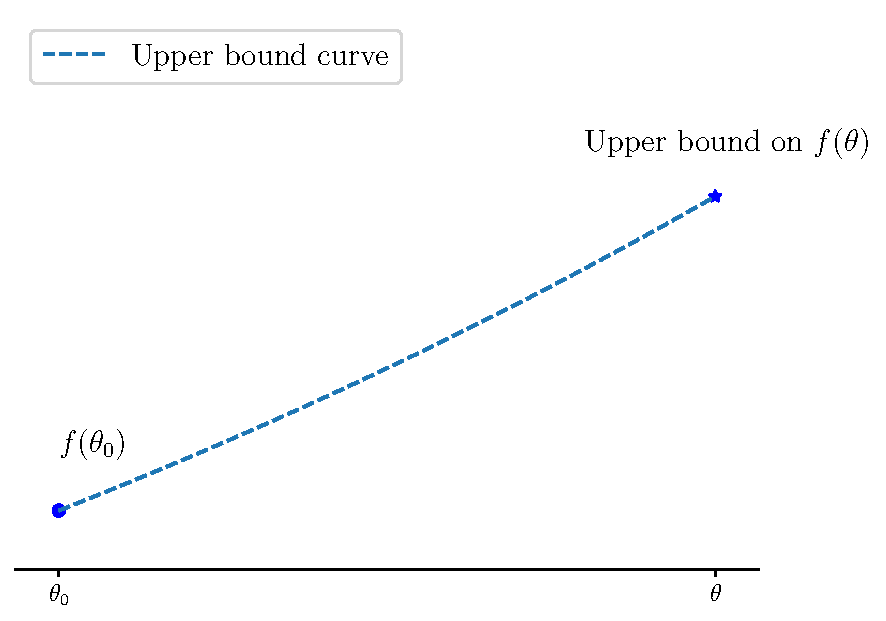
\includegraphics[width=\linewidth]{figs/cse_solution.pdf}
\end{figure} 
\end{frame}

\begin{frame}{Derivation: Begin with a Change of Measure}
Let $A := \set{x : \design(x) \text{ rejects}}$.

Then,
\begin{align*}
    f(\theta)
    &=
    \EEE_\theta\br{\indic{X \in A}}
    =
    \EEE_{\theta_0}\br{\indic{X \in A} \frac{p_\theta(X)}{p_{\theta_0}(X)}}
\end{align*}
\end{frame}

\begin{frame}{Use H\"{o}lder's Inequality!}
For any $p, q \geq 1$ such that $\frac{1}{p} + \frac{1}{q} = 1$,
\begin{align*}
    f(\theta) 
    &\leq
    \norm{\indic{X \in A}}_{L^p(P_{\theta_0})}
    \norm{\frac{p_\theta(X)}{p_{\theta_0}(X)}}_{L^q(P_{\theta_0})}
    \\&=
    f(\theta_0)^{1-\frac{1}{q}} 
    \norm{\frac{p_\theta(X)}{p_{\theta_0}(X)}}_{L^q(P_{\theta_0})}
\end{align*} 
\end{frame}

\begin{frame}{Introduce Distributional Assumptions}

Let $P_\theta$ have a density of the form:
\begin{align*}
    p_\theta(x)
    =
    \exp\sbr{g_\theta(x) - A(\theta)}
\end{align*}

By a simple calculation, one can show that
\begin{equation*}
    \norm{\frac{p_\theta(X)}{p_{\theta_0}(X)}}_{L^q(P_{\theta_0})}
    =
    \exp\sbr{
        \frac{\psi(\theta_0, \theta-\theta_0, q)}{q}
        - \psi(\theta_0, \theta-\theta_0, 1)
    }
\end{equation*} 
\begin{equation*}
    \psi(\theta_0, v, q)
    :=
    \log\EEE_{\theta_0}\br{\exp\sbr{q\pr{g_{\theta_0+v}(X)-g_{\theta_0}(X)}}}
\end{equation*} 
\end{frame}

\begin{frame}{We did it!}
For any $q \geq 1$,
\begin{align*}
    f(\theta)
    &\leq
    f(\theta_0)^{1 - \frac{1}{q}}
    \exp\sbr{\frac{\psi(\theta_0, \theta-\theta_0, q)}{q} - \psi(\theta_0, \theta-\theta_0, 1)}
\end{align*}
\end{frame}

\begin{frame}{Tilt-Bound and Special Cases}
\textbf{Tilt-Bound ($q \geq 1$):}
\begin{equation*}
    U(\theta_0, v, q, f(\theta_0))
    :=
    \underbrace{f(\theta_0)^{1 - \frac{1}{q}}}_{
    \mathclap{\textcolor{red}{\theta_0 \textbf{ info}}}
    }
    \underbrace{\exp\sbr{\frac{\psi(\theta_0, v, q)}{q} - \psi(\theta_0, v, 1)}}_{
    \mathclap{\textcolor{red}{\textbf{Curvature info}}}
    }
\end{equation*}
\textbf{Exponential family:}
\begin{equation*}
    \psi(\theta_0, v, q) 
    :=
    A(\theta_0 + qv) - A(\theta_0)
\end{equation*}
\textbf{Normal family $\set{\normal\pr{\theta, 1} : \theta \in \Theta}$:}
\begin{equation*}
    U(\theta_0, v, q, f(\theta_0))
    :=
    f(\theta_0)^{1 - \frac{1}{q}} 
    \exp\sbr{\frac{(q - 1) v^2}{2}}
\end{equation*}
\end{frame}

\begin{frame}{Optimize over $q$!}
\begin{align*}
    f(\theta_0 + v) 
    &\leq 
    U(\theta_0, v, q, f(\theta_0))
    \quad \forall q \geq 1
    \\\\ \implies
    f(\theta_0 + v)
    &\leq
    \underbrace{%
    \inf\limits_{q \geq 1}
    U(\theta_0, v, q, f(\theta_0))}_{
    \mathclap{\textcolor{red}{\textbf{Optimized Tilt-Bound}}}
    }
\end{align*}  
\end{frame}

\begin{frame}{How to optimize over $q$?}
\begin{itemize}
    \item Tilt-Bound is \textbf{quasi-convex} in $q$!
    \item Very \textbf{simple, fast} 
        $O(\log(\epsilon^{-1}))$ algorithm
        with \textbf{guaranteed convergence}.
\end{itemize}    
\begin{theorem}[Quasi-convex in $q$]
Fix any $\theta_0 \in \Theta \subseteq \R^d$,
a set $S \subseteq \R^d$,
and $a \geq 0$.
Assume that for all $v \in S$,
$\Delta(v, X) := g_{\theta_0 + v}(X) - g_{\theta_0}(X)$
is not constant $P_{\theta_0}$-a.s..
Then, $q \mapsto \sup\limits_{v \in S} U(\theta_0, v, q, a)$ 
is quasi-convex.
Moreover, it is strict if $a > 0$, $S$ is finite, 
and not identically infinite, respectively.
\end{theorem}
\end{frame}

\begin{frame}{Demonstrating the Tilt-Bound on the One-Sided Z-Test}
\begin{figure}
    \centering
    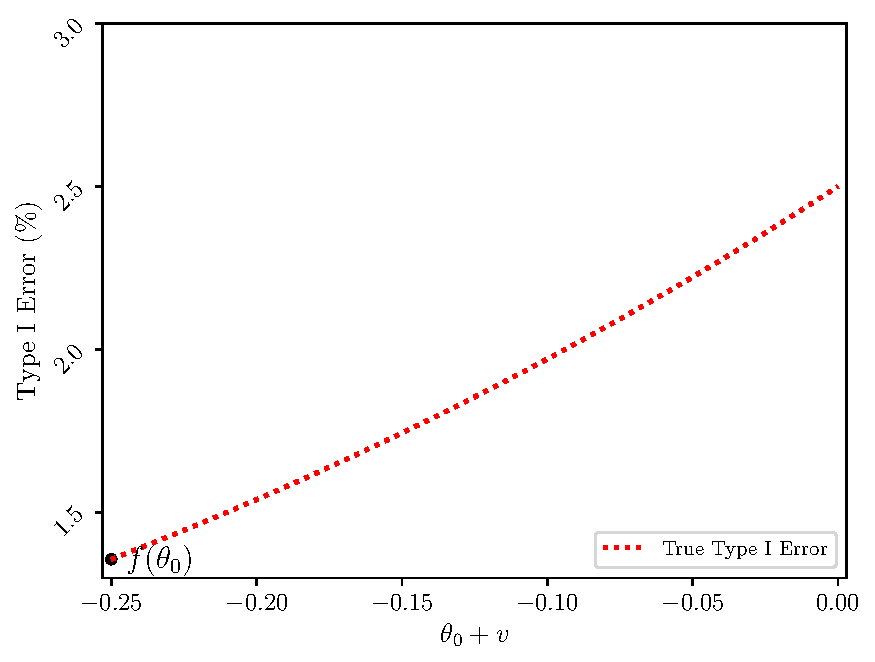
\includegraphics[width=0.85\linewidth]{figs/greens_up_tie.pdf}
\end{figure}
\begin{itemize}
    \item $X \sim \normal\pr{\theta, 1}$, $\Theta = [-0.25, 0]$.
    \item $\design(X)$: reject if $X > z_{1-\alpha}$.
\end{itemize}
\end{frame}

\begin{frame}{The Tilt-Bound for a Particular $q$}
\begin{figure}
    \centering
    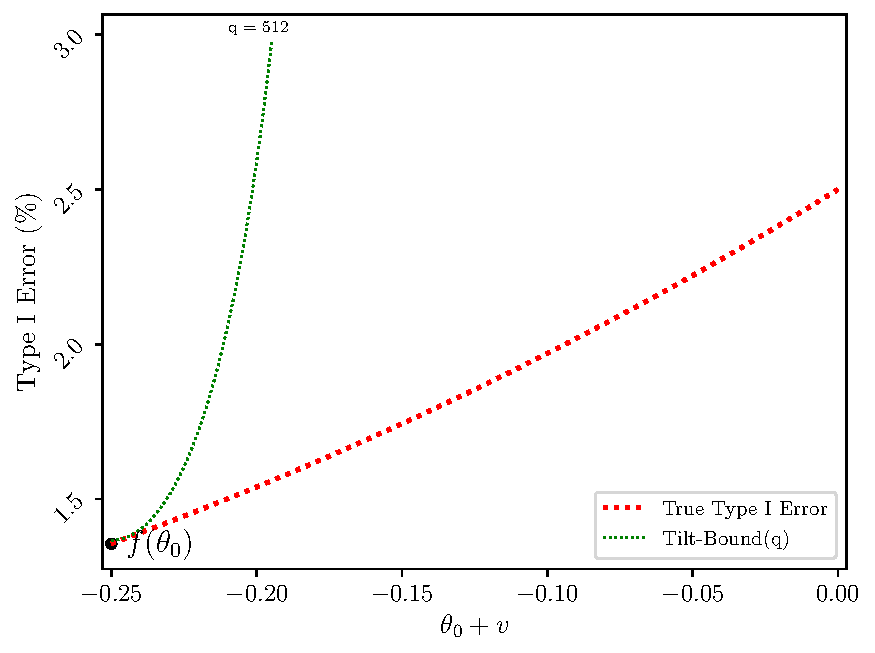
\includegraphics[width=0.85\linewidth]{figs/greens_up_one_q.pdf}
\end{figure} 
\begin{equation*}
    U(\theta_0, v, q, f(\theta_0))
    =
    f(\theta_0)^{1 - \frac{1}{q}} 
    \exp\sbr{\frac{(q - 1) v^2}{2}}
\end{equation*}
\end{frame}

\begin{frame}{The Tilt-Bound for Many $q$s}
\begin{figure}
    \centering
    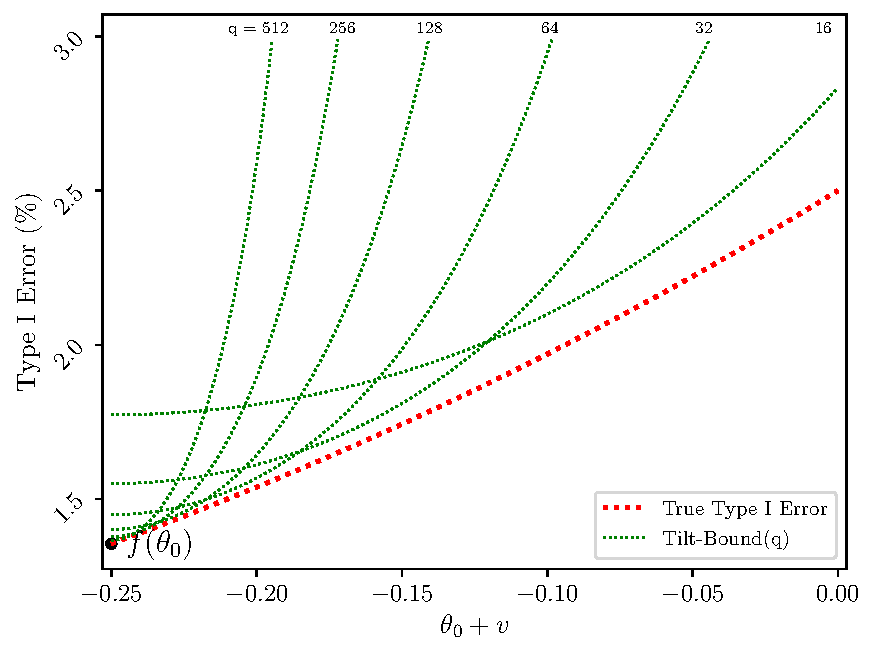
\includegraphics[width=0.85\linewidth]{figs/greens_up_all_q.pdf}
\end{figure} 
\begin{equation*}
    U(\theta_0, v, q, f(\theta_0))
    =
    f(\theta_0)^{1 - \frac{1}{q}} 
    \exp\sbr{\frac{(q - 1) v^2}{2}}
\end{equation*}
\end{frame}

\begin{frame}{The Optimized Tilt-Bound is Tight}
\begin{figure}
    \centering
    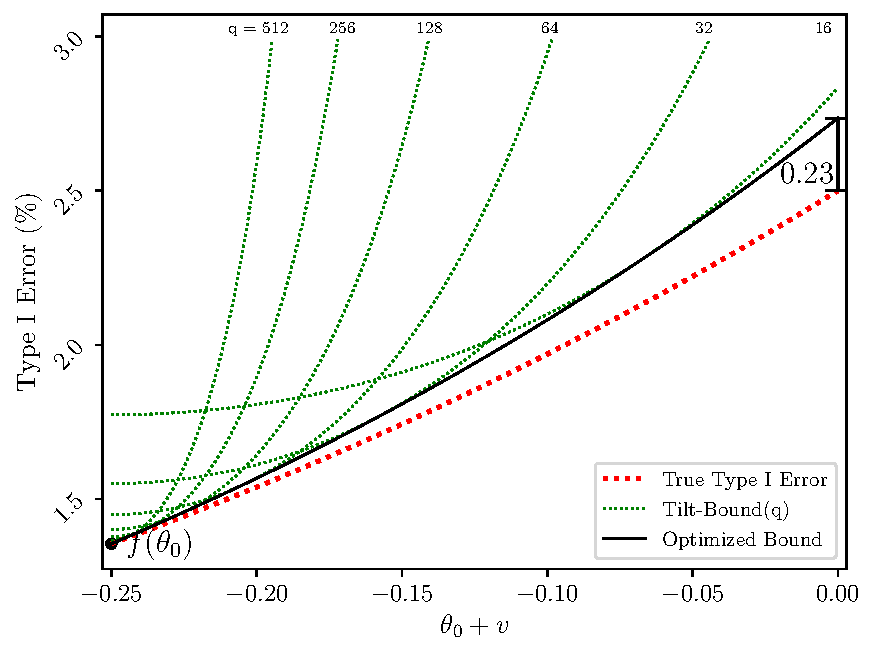
\includegraphics[width=0.85\linewidth]{figs/greens_up.pdf}
\end{figure} 
\begin{equation*}
 \inf\limits_{q \geq 1} U(\theta_0, v, q, f(\theta_0))
\end{equation*}
\end{frame}

\begin{frame}{Tilt-Bound Summary}
\begin{itemize}
    \item Tilt-Bound is a \textbf{deterministic} bound.
    \item Tight over small to medium distances.
    \item Valid for \textbf{any rejection set}.
    \item Depends on Type I Error at the 
    \textbf{initial point $\theta_0$} and 
    the \textbf{distributional family $P_\theta$} 
    (which implicitly accounts for the sample size).
\end{itemize}
\end{frame}